\documentclass{article}

\usepackage[margin=0.8in]{geometry}
\usepackage{polski}
\usepackage[utf8x]{inputenc}
\usepackage[hidelinks]{hyperref}
\usepackage{amsmath}
\usepackage{graphicx}
\usepackage[export]{adjustbox}
\usepackage{float}
\usepackage{subcaption}
\usepackage{listings}
\usepackage{color}

\hypersetup{
	colorlinks,
 	citecolor=black,
 	filecolor=black,
  	linkcolor=black,
  	urlcolor=black
}

\lstset{
	language=Python,													% the language of the code
	basicstyle=\small\ttfamily,
	numbers=left,
	numberstyle=\tiny,
	frame=tb,
	tabsize=4,
	columns=fixed,
	showstringspaces=false,
	showtabs=false,
	keepspaces,
	breaklines=true,											% sets automatic line breaking
	postbreak=\mbox{\textcolor{red}{$\hookrightarrow$}\space},
	commentstyle=\color{green},
	keywordstyle=\color{blue},
	stringstyle=\color{red},
	extendedchars=true,
	inputencoding=utf8x
}

\begin{document}

\begin{titlepage}
	\newcommand{\HRule}{\rule{\linewidth}{0.5mm}}
	\center
	
	%------------------------------------------------
	%	Headings
	%------------------------------------------------
	\textsc{\LARGE Politechnika Wrocławska}\\[1.5cm] 	
	\textsc{\Large Wydział Elektroniki}\\[0.5cm] 
	\textsc{\large Niezawodność i diagnostyka układów cyfrowych}\\[0.5cm] 
	
	%------------------------------------------------
	%	Title
	%------------------------------------------------
	\HRule\\[0.4cm]
	{\huge\bfseries Analiza metod modulacji PSK i APSK}\\[0.4cm]
	\HRule\\[1.5cm]
	
	%------------------------------------------------
	%	Author(s)
	%------------------------------------------------
	\begin{minipage}{0.4\textwidth}
		\begin{flushleft}
			\large
			\textit{Skład zespołu}\\
			Maja \textsc{Bojarska}\\
			Wojciech \textsc{Sadlik}\\
			Wojciech \textsc{Śliwa}\\
		\end{flushleft}
	\end{minipage}
	~
	\begin{minipage}{0.4\textwidth}
		\begin{flushright}
			\large
			\textit{Prowadzący}\\
			mgr inż. Szymon \textsc{Datko}
		\end{flushright}
	\end{minipage}
	
	%------------------------------------------------
	%	Date
	%------------------------------------------------
	\vfill\vfill\vfill 
	{\large\today} 
	\vfill 
	
\end{titlepage}

%	Main content
\section{Wstęp}
	Celem projektu było zbadanie skuteczności metod modulacji PSK oraz APSK. Stworzony został model systemu komunikacyjnego, zawierający takie elementy składowe jak modulator i demodulator oraz kanał transmisyjny z zakłóceniami o zmiennym poziomie. Efektywność danej metody modulacji jest określona za pomocą wartości BER i SNR w zależności od natężenia szumu oraz typu modulacji.\\
	Zostały przeprowadzone następujące testy:
	\begin{enumerate}
		\item Wartości SNR i BER dla QPSK w funkcji wariancji rozkładu normalnego; szum gaussowski; wariancja z przedziału od 0,1 do 2,0.
		\item Wartości SNR i BER dla 64-PSK w funkcji wariancji rozkładu normalnego; szum gaussowski; wariancja z przedziału od 0,01 do 1,0.
		\item Wartości SNR i BER dla QPSK w funkcji amplitudy szumu; szum o rozkładzie równomiernym; amplituda z przedzału od 0,1 do 2,0.
		\item Wartości SNR i BER dla 64-PSK w funkcji amplitudy szumu; szum o rozkładzie równomiernym; amplituda z przedzału od 0,01 do 1,0.
		\item Wartości SNR i BER dla QAPSK w funkcji wariancji rozkładu normalnego; szumu gaussowski; wariancja z przedziału od 0,1 do 2,0.
		\item Porównanie skuteczności modulacji QPSK i QAPSK; szumu gaussowski; wariancja z przedziału od 0,1 do 2,0.
		\item Porównanie skuteczności BPSK, QPSK, 8-PSK, 16-PSK, 32-PSK, 64-PSK, 128-PSK, 256-PSK, 512-PSK, 1024-PSK; szum gaussowski, wariancja rozkładu normalnego równa 0,5.
	\end{enumerate}

\section{Wprowadzenie}
	\subsection{Modulacja cyfrowa}
		Modulacja to proces dopasowywanie transmitowanego sygału do fali nosnej, poprzez zmianę jego parametrów. Tak przetworzony sygnał może być natępnie przesłany kanałem transmisyjnym. Celem modulacji jest m.in. zwiększenie efektywności przesyłu danych. Odpowiednio przetworzony sygnał umożliwia przesłanie kilku bitów informacji w jednym okresie fali nośnej. Oczywiście długość symbolu wpływa na odporność transmisji na zakłócenia.

	\subsection{Kluczowanie fazy}
		Kluczowanie fazy, PSK (ang. \textit{Phase-Shift keying}) --- to rodzaj modulacji cyfrowej, polegający na dyskretnych zmianach fazy sygnału. Każdy z podrodzajów PSK posiada skończoną liczbę faz, którym przypisany jest unikalny ciąg binarny. Najczęśniej wszystkie symbole są identycznej długości $2^{n}$, gdzie $n > 0$. PSK można podzielić na:
		\begin{itemize}
			\item BPSK (ang. \textit{Binary PSK}) --- występują dwia przesunięcia fazy, a słowo ma długość jednego bitu,
			\item QPSK (ang. \textit{Quadrature PSK}) --- występują cztery przesunięcia fazy, a słowo ma długość dwóch bitów,
			\item n-PSK -- występuje n przesunięć fazy, a słowo ma długość $log_{2}n$ bitów.
		\end{itemize}
		Działanie modulacji PSK można w jasny sposób przedstawić za pomocą diagramu konstelacji. Poszczególne fazy, wraz z udpowiadającymi im ciągami dwójkowymi, umieszczone są na płaszczyźnie zespolonej.
		%-fig. PSK diagram konstelacji - placeholder
		\begin{figure}[H]
			\centering
			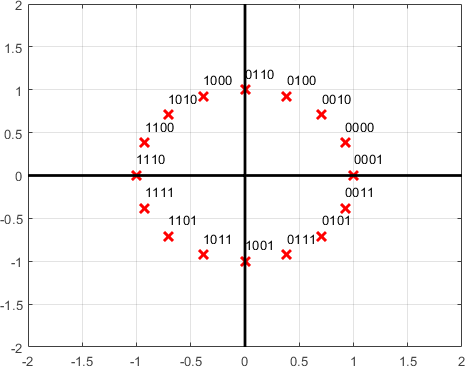
\includegraphics[width=0.8\linewidth]{img/intro_psk_constelation.png}
			\caption{Diagram konstelacji 16-PSK}
			\label{fig:intro_psk_constelation}
		\end{figure}

	\subsection{Jednoczesne kluczowanie fazy i amplitudy}
		Kluczowanie fazy i amlitudy, APSK (ang. \textit{Amplitude and Phase-Shift Keying}) --- to rodzaj modulacji cyfrowej, polegający na dyskretnych zmianach zarówno fazy fali nośnej, jak i amplitudy. Innymi słowy jest to połączenie modulacji ASK i PSK w celu zwiększenia liczby symboli. Działanie modulacji APSK można w jasny sposób przedstawić za pomocą diagramu konstelacji. Poszczególne fazy, wraz z udpowiadającymi im ciągami dwójkowymi, umieszczone są na płaszczyźnie zespolonej.
		\begin{figure}[H]
			\centering
			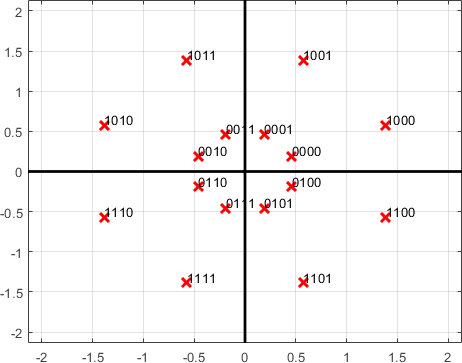
\includegraphics[width=0.8\linewidth]{img/intro_apsk_constelation.png}
			\caption{Diagram konstelacji 16-APSK}
			\label{fig:intro_apsk_constelation}
		\end{figure}

	\subsection{Współczynniki efektywności}
		\begin{itemize}
			\item Długość słowa --- określa liczbę bitów ciągu wejściowego, która może zostać przesłana w jednym okresie fali nośnej.
			\item BER (ang. \textit{Bit Error Rate}), współczynnik błędnych bitów --- to wskaźnik określający prawdopodobieństwo wystąpięnia przekłamania bitu informacji w strumieniu przesyłanych danych.
			\item SNR (ang. \textit{Signal-to-Noise Ratio}), stosunek sygnału do szumu --- to miara porównujące poziom sygnału przenoszącego informację do poziomu szumu.
		\end{itemize}
		

\section{Opis zastosowanego modelu}
	\begin{itemize}
		\item Transmitowanymi danymi są losowe ciągi bitów o określonej długości.
		\item Modulacja polega na podzieleniu ciągu wejściowego na segmentu, których długość jest zależna od metody modulacji. Na przykład dla 16-PSK będą to 4 bity na segment. Następnie segmenty są zamieniane na odpowiadające im wartości fazy -- punkty na płaszyźnie zespolonej.
		\item Do wektora zmodulowanego sygnału dodawany jest szum. Ta operacja symuluje przysył danych przez medium transmisyjne. Model uwzględnia szum o rozkładzie normalnym, równomiernym oraz von Misesa. Parametry zakłóceń mogą być regulowane.
		\item Demodulacja polega na odtworzeniu z wektora zaszumionego sygnału ciągu bitów wyjściowych.
	\end{itemize}

	%-fig. Model schemat blokowy
	\begin{figure}[H]
		\centering
		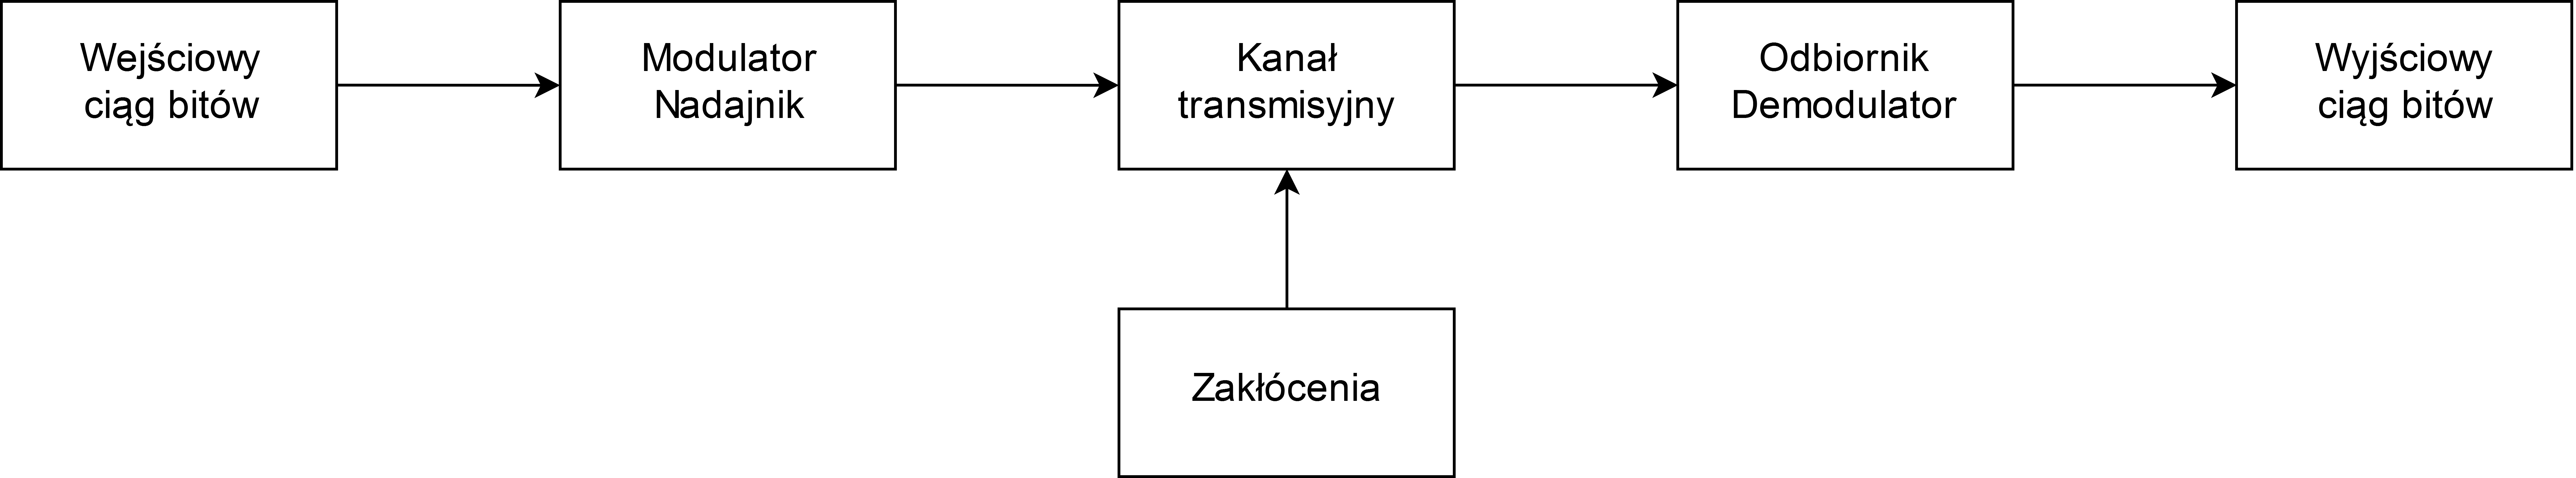
\includegraphics[width=\linewidth]{img/desc_model_block.png}
		\caption{Schemat blokowy modelu systemu komunikacyjnego}
		\label{fig:desc_model_block}
	\end{figure}

\section{Opis eksperymentu}
	Na potrzeby eksperymentu została stworzona aplikacja w języku Python. Udostępnia ona szereg funkcji umożliwiających sprawne przeprowadzanie testów. Pojedynczą sesję badawczą można stresicić w następującej liście kroków:
	\begin{enumerate}
		\item Wybranie długości ciągu transmitowanych danych.
		\item Wybranie rozkładu szumu oraz parametrów. Zaimplementowne rozkłady to: jednostajny (parametrem jest amplituda), normalny (parametrami są wartość oczekiwana i wariancja), von Misesa (parametrem jest dyspersja).
		\item Określenie typu modulacji PSK lub APSK. 
		\item Ustawienie liczby różnych symulacji.
	\end{enumerate} 
	Program po wykonaniu obliczeń umożliwia przeglądanie wyników dla poszczególnych symulacji. Zaszumiony zmodulowany wykres jest wyświetlany w formię wykresu wskazowego. Rezultaty badań można następnie zapisać do pliku z rozszerzeniem csv.

	Dla wszystkich pomiarów z sekcji \textbf{Wyniki badań} przyjęto następujące założenia: długość ciągu wejściowego dla każdego pomiaru wynosi 4096 bitów; każdą symulację transmisji wykonano 100 razy, a otrzymane wyniki zostały uśrednione przed naniesieniem na wykres; wartość oczekiwana w rozładnie normalnym jest zawsze równa 0.

\section{Implementacja}
	Funkcje programu realizujące modulację i demodulację pochodzą z zewnętrznego modułu o nazwie \textit{Komm}.
	
	\noindent Zaszumianie polega na wylosowaniu wektora liczb zespolonych, której długość jest równa długości listy zawierającej sygnał zmodulowany. Następnie oba ciągi są sumowane.
	
	\noindent Za obliczenie BER odpowiada poniższa funkcja:
	\begin{lstlisting}
def bit_error_rate(bits1, bits2, precision=4):
	ber = 0
	if len(bits1) != 0:
		counter = 0
		for i in range(len(bits1)):
			if bits1[i] != bits2[i]:
				counter += 1
		ber = round(counter / len(bits1), precision)
	return ber
	\end{lstlisting}
	\noindent Argumentami wywołania są ciągi przed i po transmisji. Działanie polega na wyliczeniu stosunku liczby przekłamanych bitów do całkowitej długości sygnału.\\

\newpage
	\noindent Za obliczenie SNR odpowiada następująca funkcja:
	\begin{lstlisting}
def signal_noise_ratio(signal_clear, noise):
	snr_sum = 0
	if len(signal_clear) != 0:
		for i in range(len(signal_clear)):
			snr_sum += abs(signal_clear[i] / noise[i])
		snr = snr_sum / len(signal_clear)
	return snr
	\end{lstlisting}
	\noindent Argumentami wywołanie są: ciąg zmodulowanego sygnału oraz wektor szumu. 

\newpage
\section{Wyniki badań}
	\subsection{Modulacja PSK, szum zgodny z rozkładem normalnym}
		\begin{figure}[H]
			\centering
			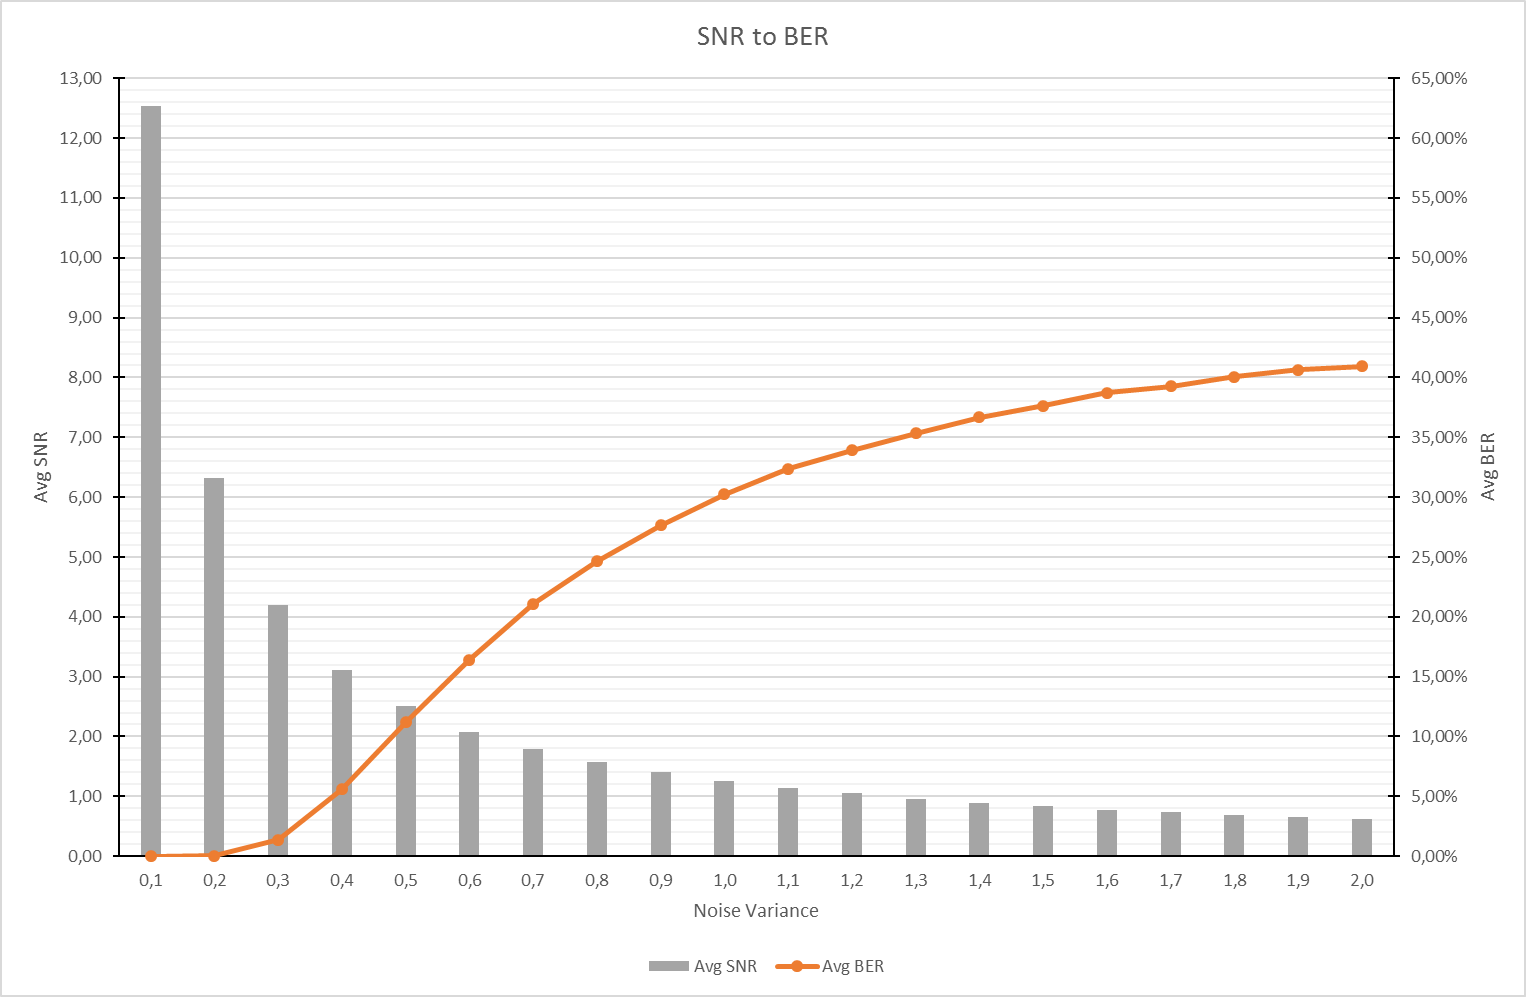
\includegraphics[width=0.8\linewidth]{img/chart/qpsk_snr_ber.png}
			\caption{QPSK, BER i SNR w funkcji wariancji szumu}
			\label{fig:qpsk_snr_ber}
		\end{figure}

		\begin{figure}[H]
			\centering
		  	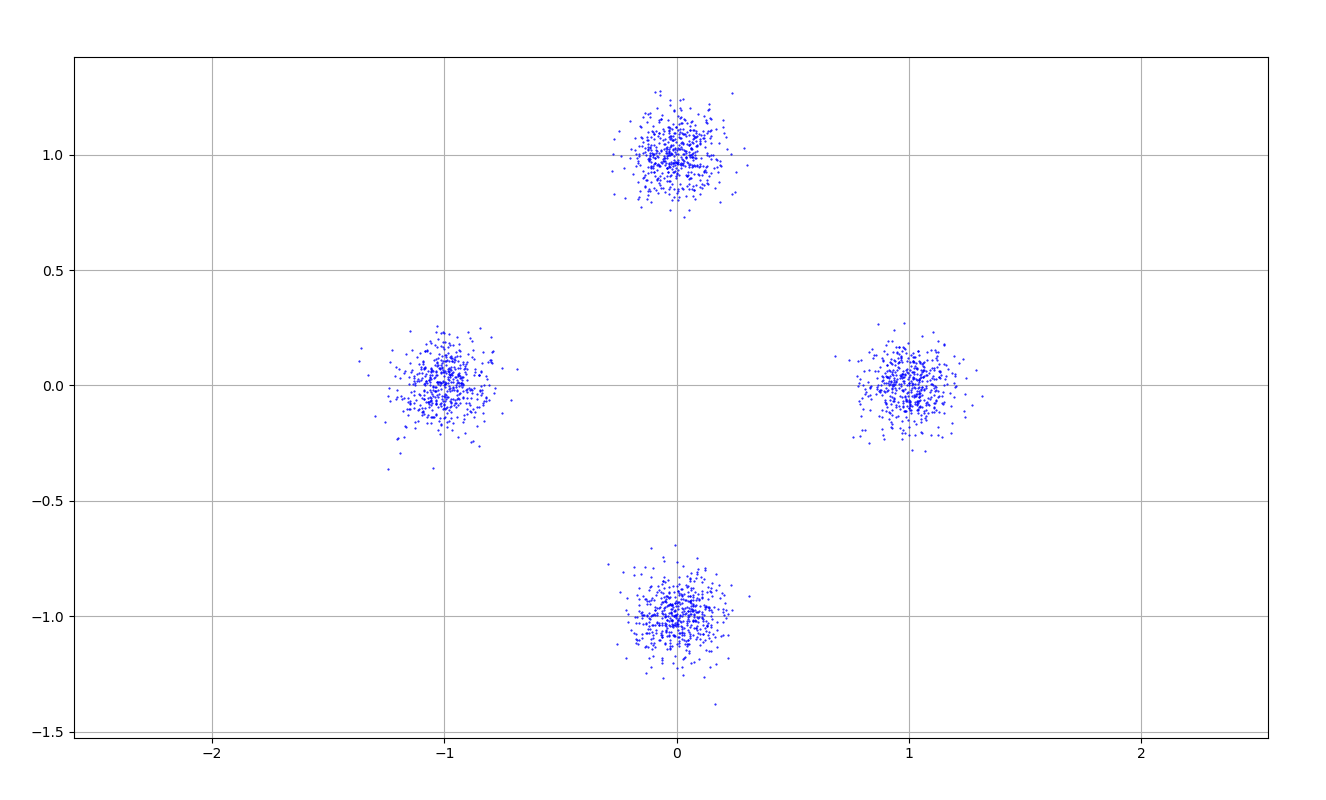
\includegraphics[width=0.8\linewidth]{img/chart/qpsk_var01_const.png}
		  	\caption{QPSK, przykładowy wykres wskazowy, wariancja szumu równa 0,1}
			\label{fig:qpsk_const}
		\end{figure}

		\begin{figure}[H]
			\centering
			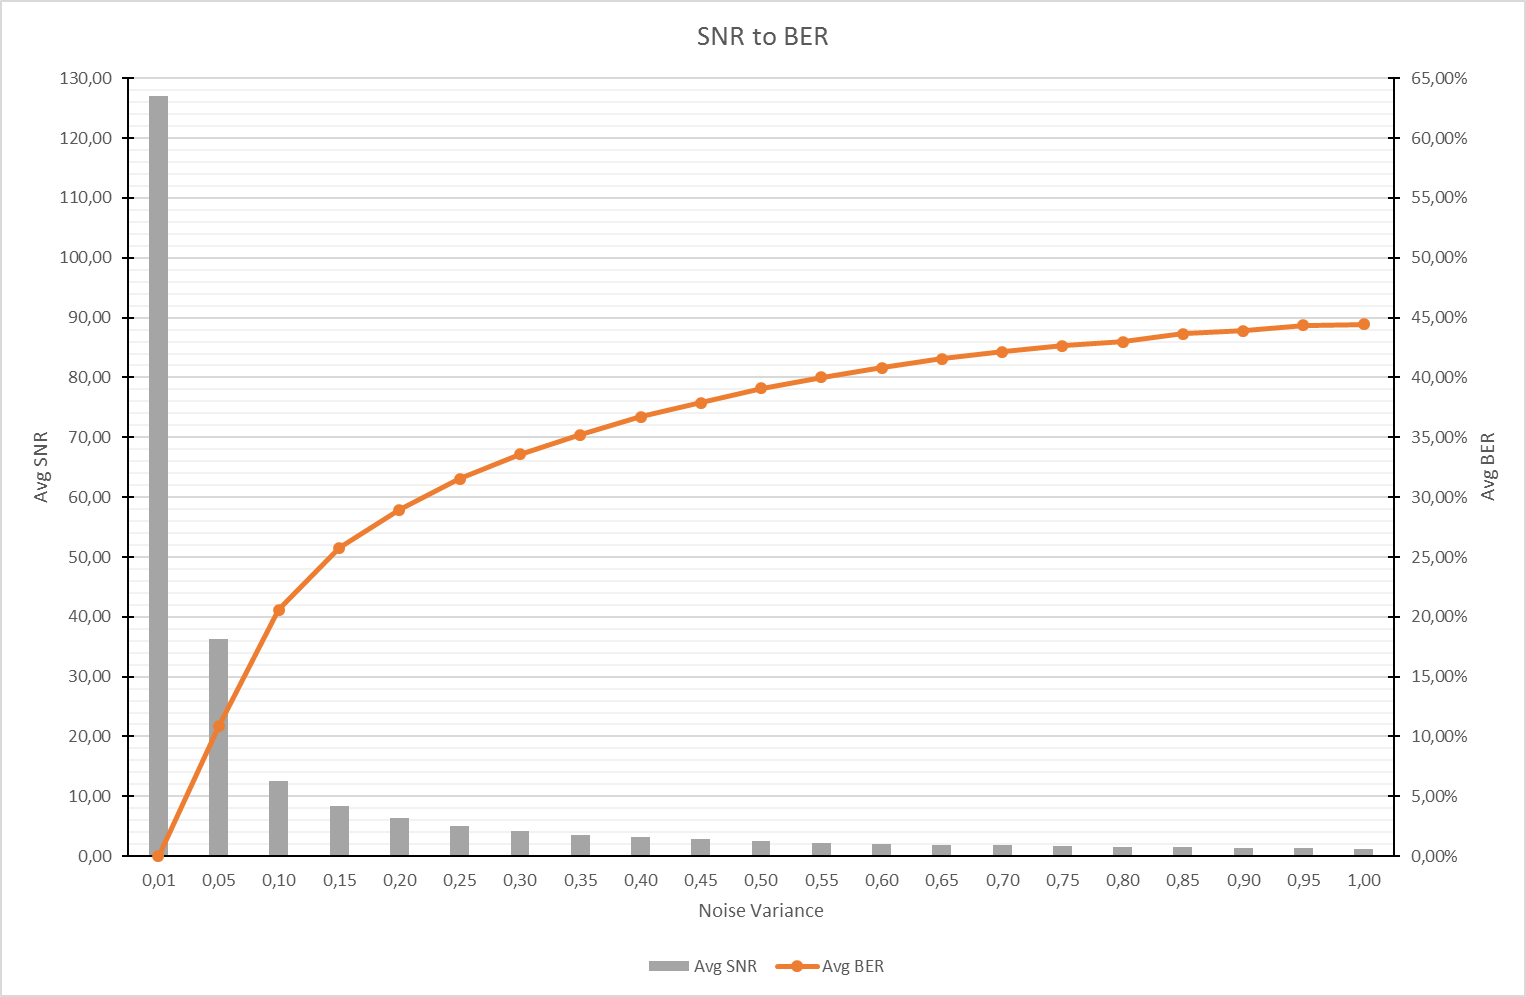
\includegraphics[width=0.8\linewidth]{img/chart/64psk_snr_ber.png}
			\caption{64-PSK, BER i SNR w funkcji wariancji szumu}
			\label{fig:64psk_snr_ber}
		\end{figure}

	\subsection{Modulacja PSK, szum zgodny z rozkładem równomiernym}
		\begin{figure}[H]
			\centering
			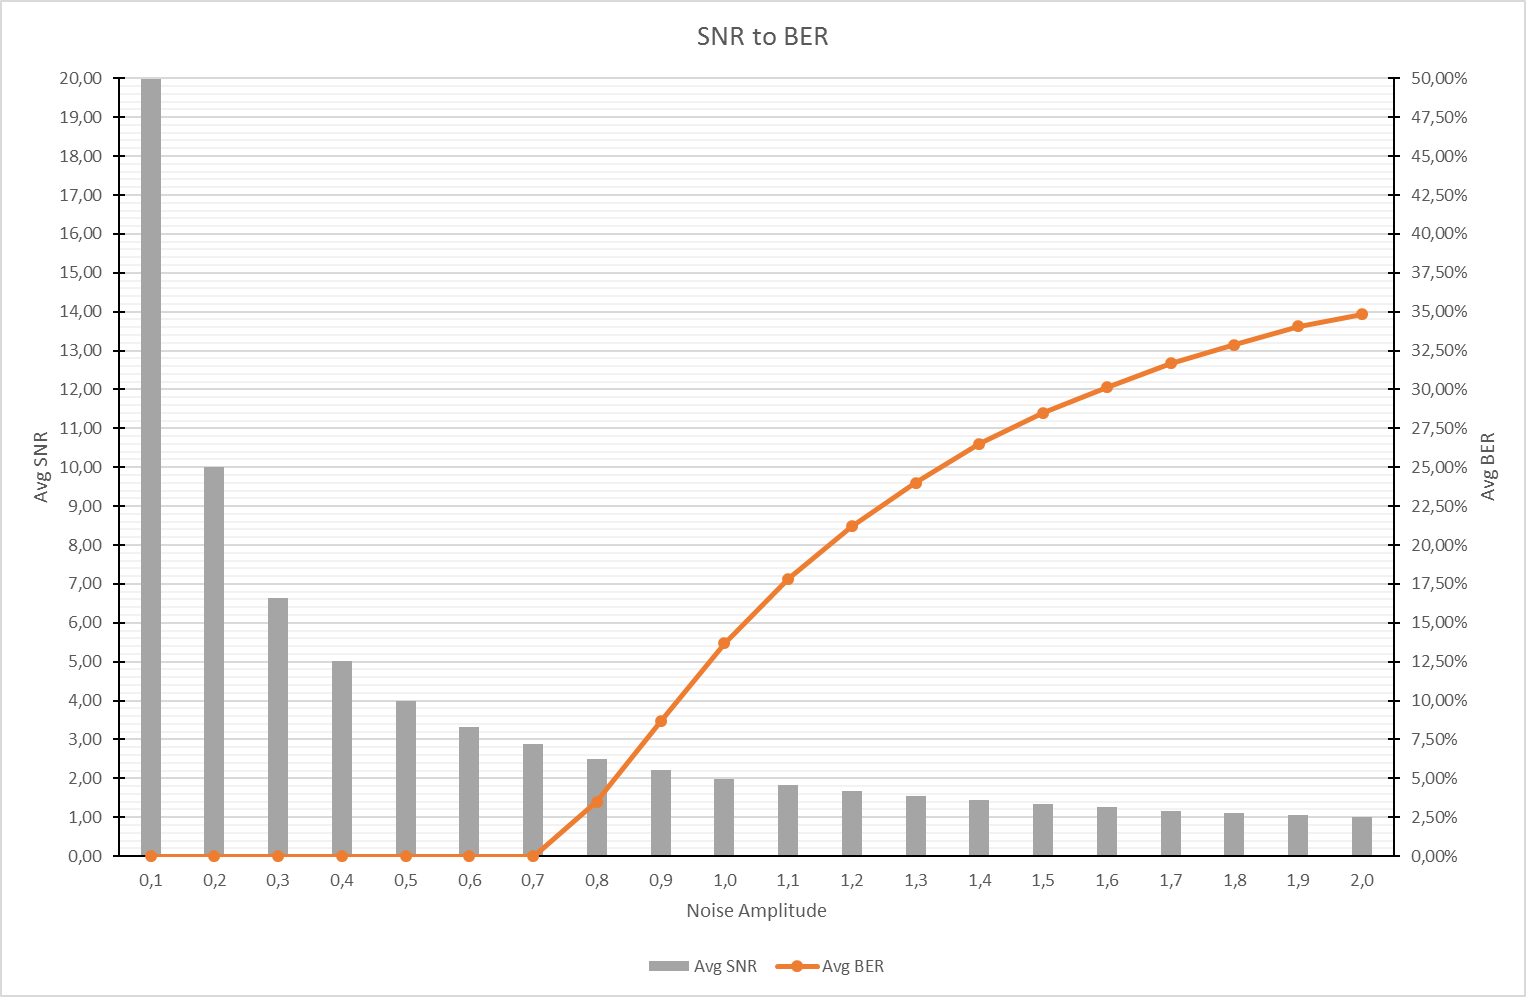
\includegraphics[width=0.8\linewidth]{img/chart/qpsk_snr_ber_uni.png}
			\caption{QPSK, BER i SNR w funkcji amplitudy szumu}
			\label{fig:qpsk_snr_ber_uni}
		\end{figure}

		\begin{figure}[H]
			\centering
			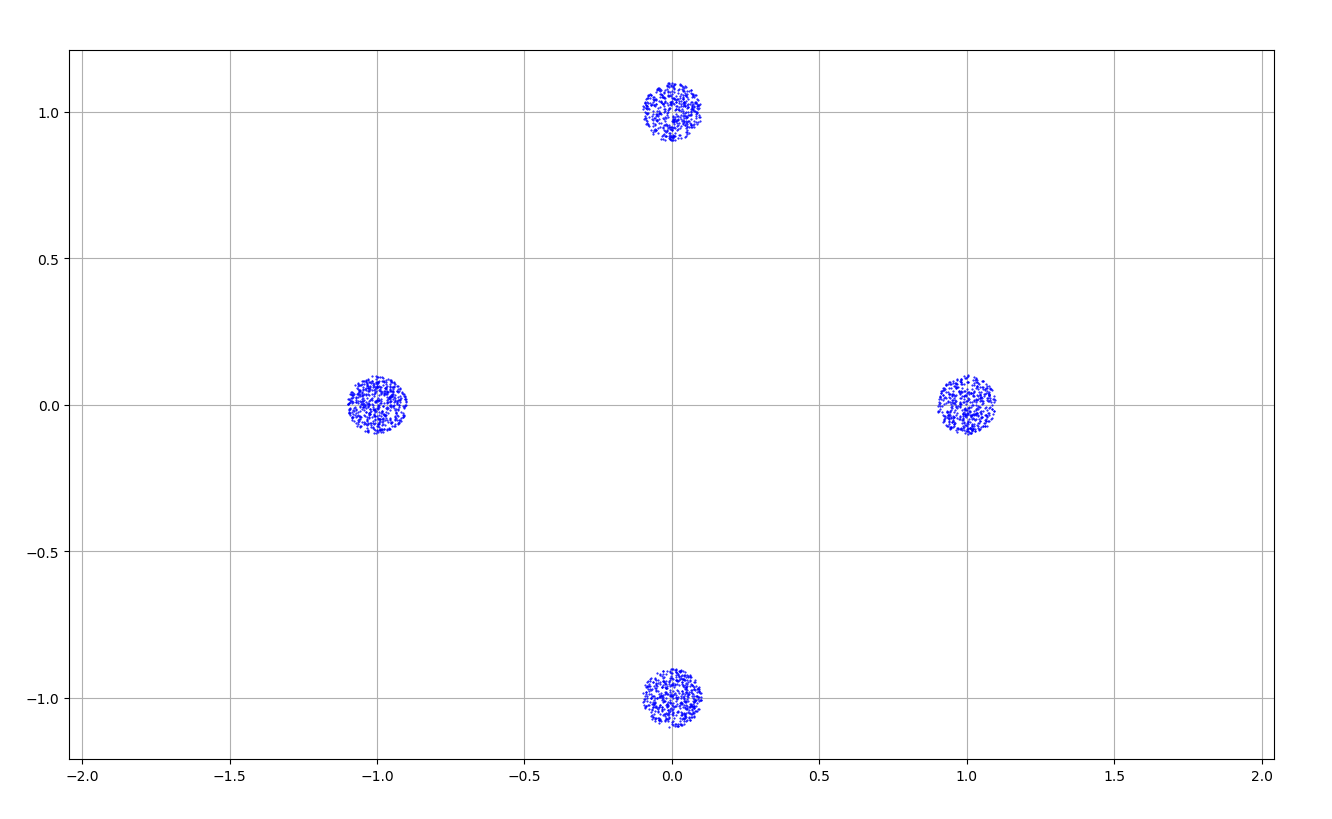
\includegraphics[width=0.8\linewidth]{img/chart/qpsk_var01_const_uni.png}
			\caption{QPSK, przykładowy wykres wskazowy, amplituda szumu równa 0,1}
			\label{fig:qpsk_const_uni}
		\end{figure}

		\begin{figure}[H]
			\centering
			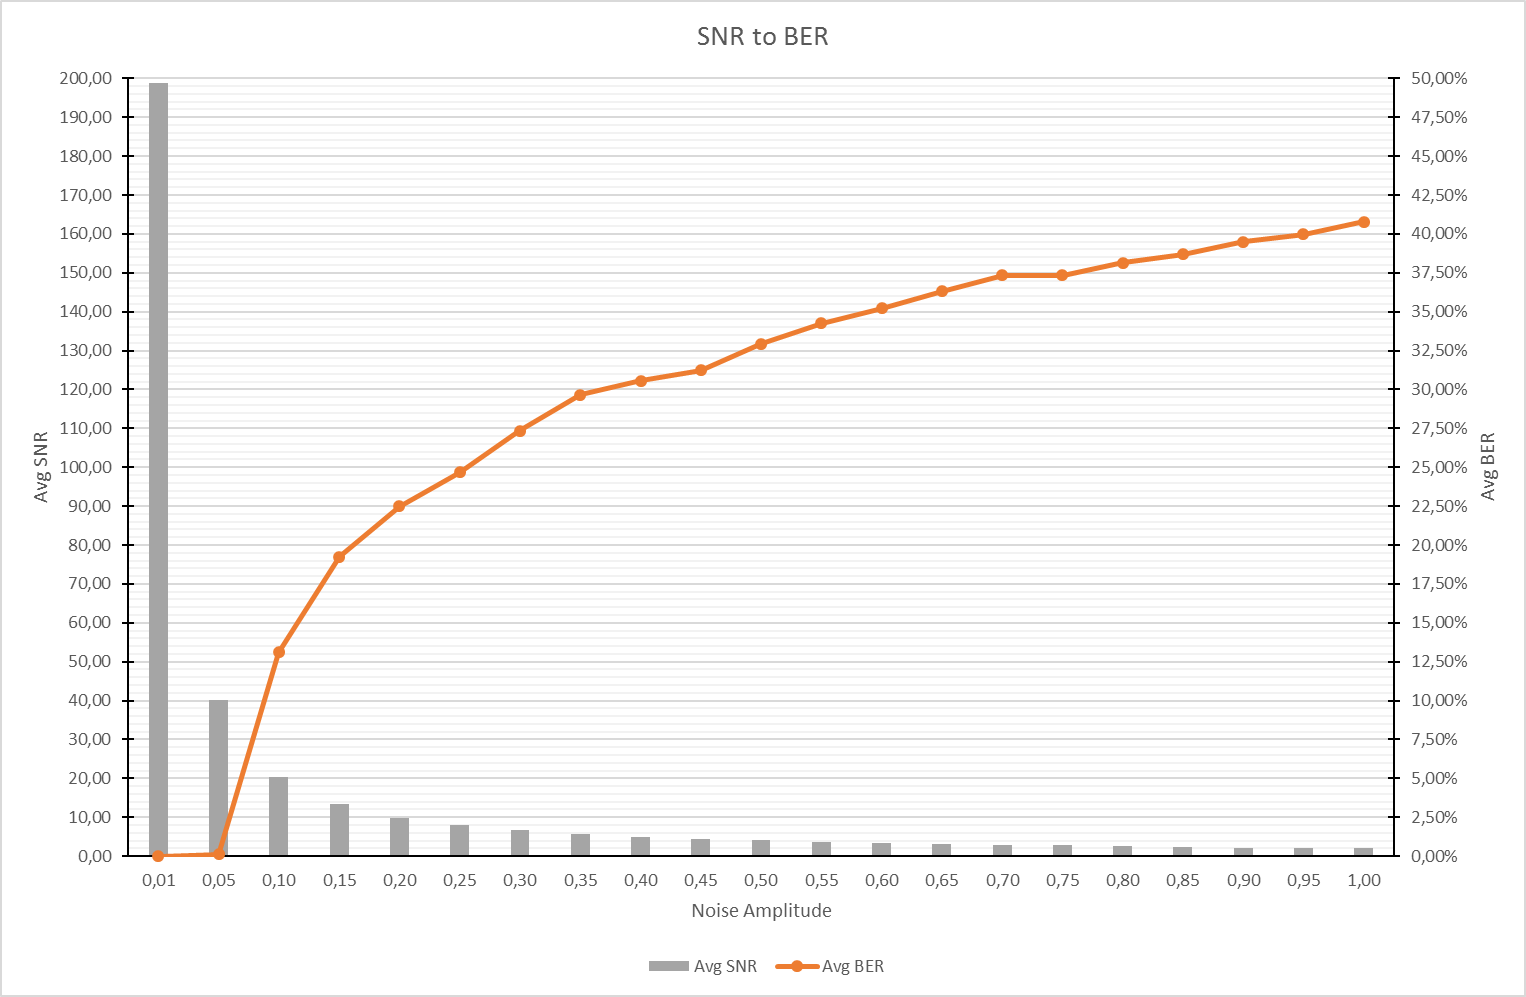
\includegraphics[width=0.8\linewidth]{img/chart/64psk_snr_ber_uni.png}
			\caption{64-PSK, BER i SNR w funkcji amplitudy szumu}
			\label{fig:64psk_snr_ber_uni}
		\end{figure}

	\subsection{Modulacja QAPSK, szum zgodny z rozkładem normalnym}
		\begin{figure}[H]
			\centering
			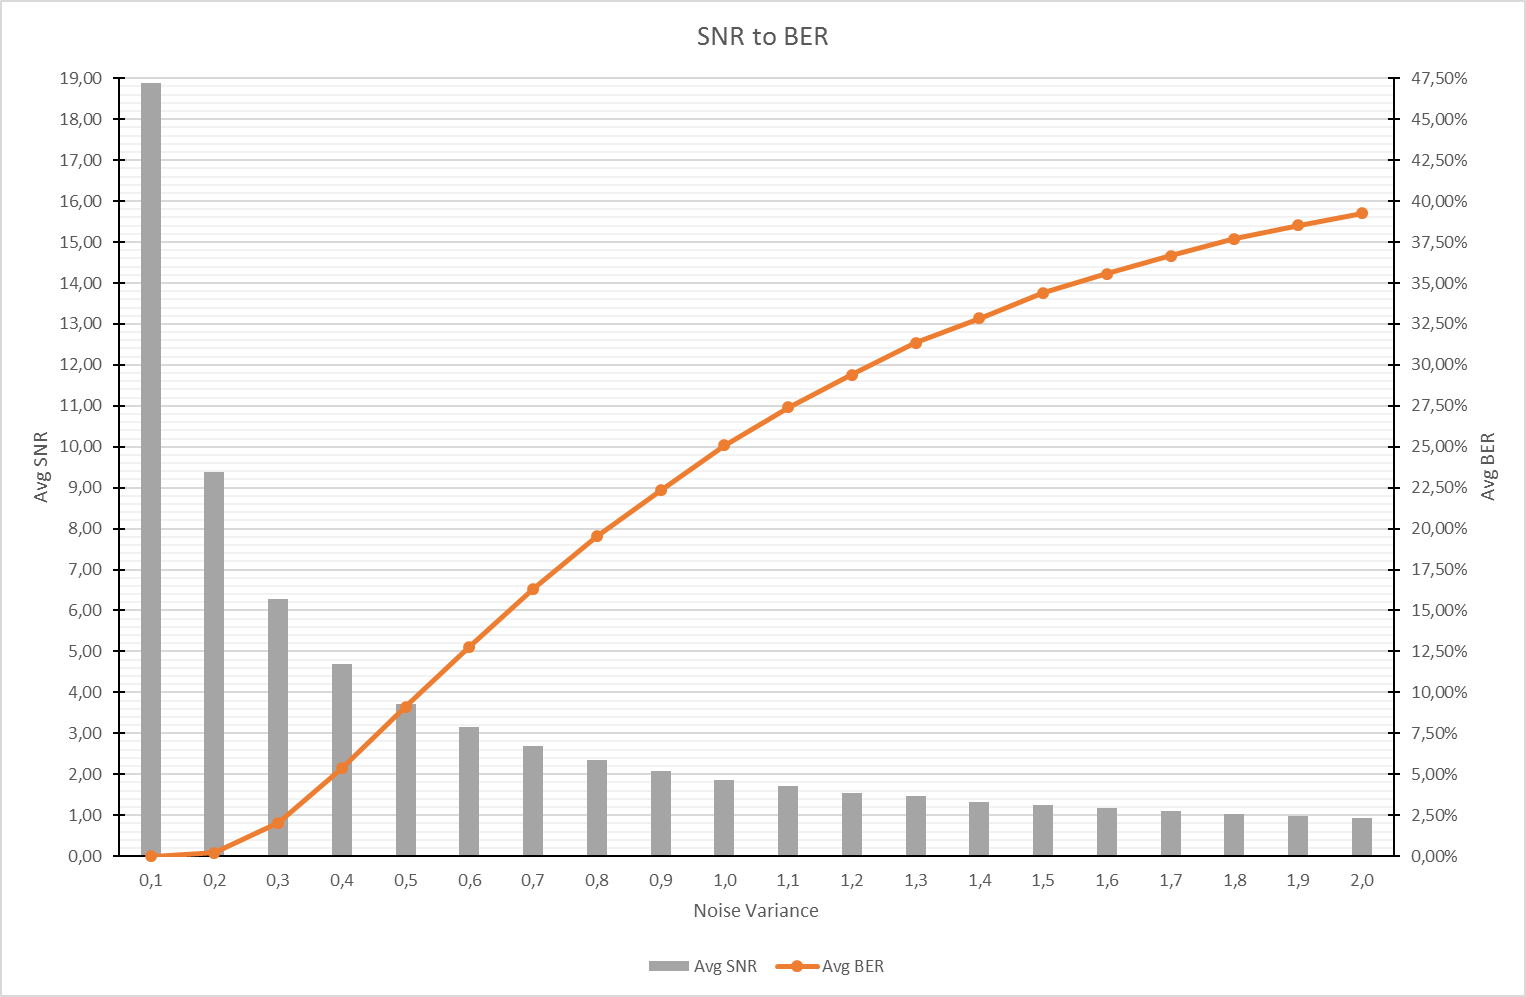
\includegraphics[width=0.8\linewidth]{img/chart/qapsk_snr_ber.png}
			\caption{QAPSK, BER i SNR w funkcji amplitudy szumu}
			\label{fig:qapsk_snr_ber}
		\end{figure}

		\begin{figure}[H]
			\centering
			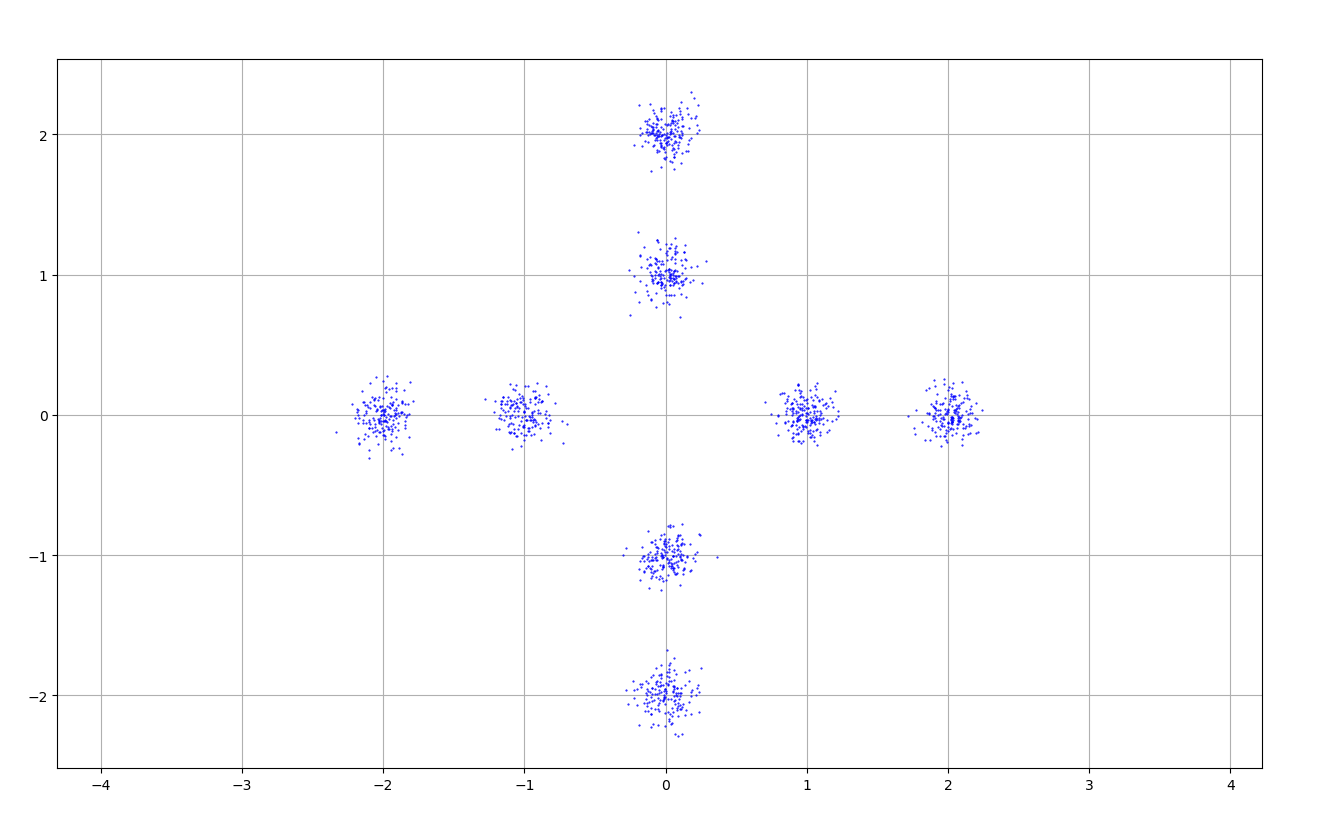
\includegraphics[width=0.8\linewidth]{img/chart/qapsk_var01_const.png}
			\caption{QAPSK, przykładowy wykres wskazowy, wariancja szumu równa 0,1}
			\label{fig:qapsk_const}
		\end{figure}

	\subsection{Porównanie modulacji QPSK i QAPSK}
		\begin{figure}[H]
			\centering
			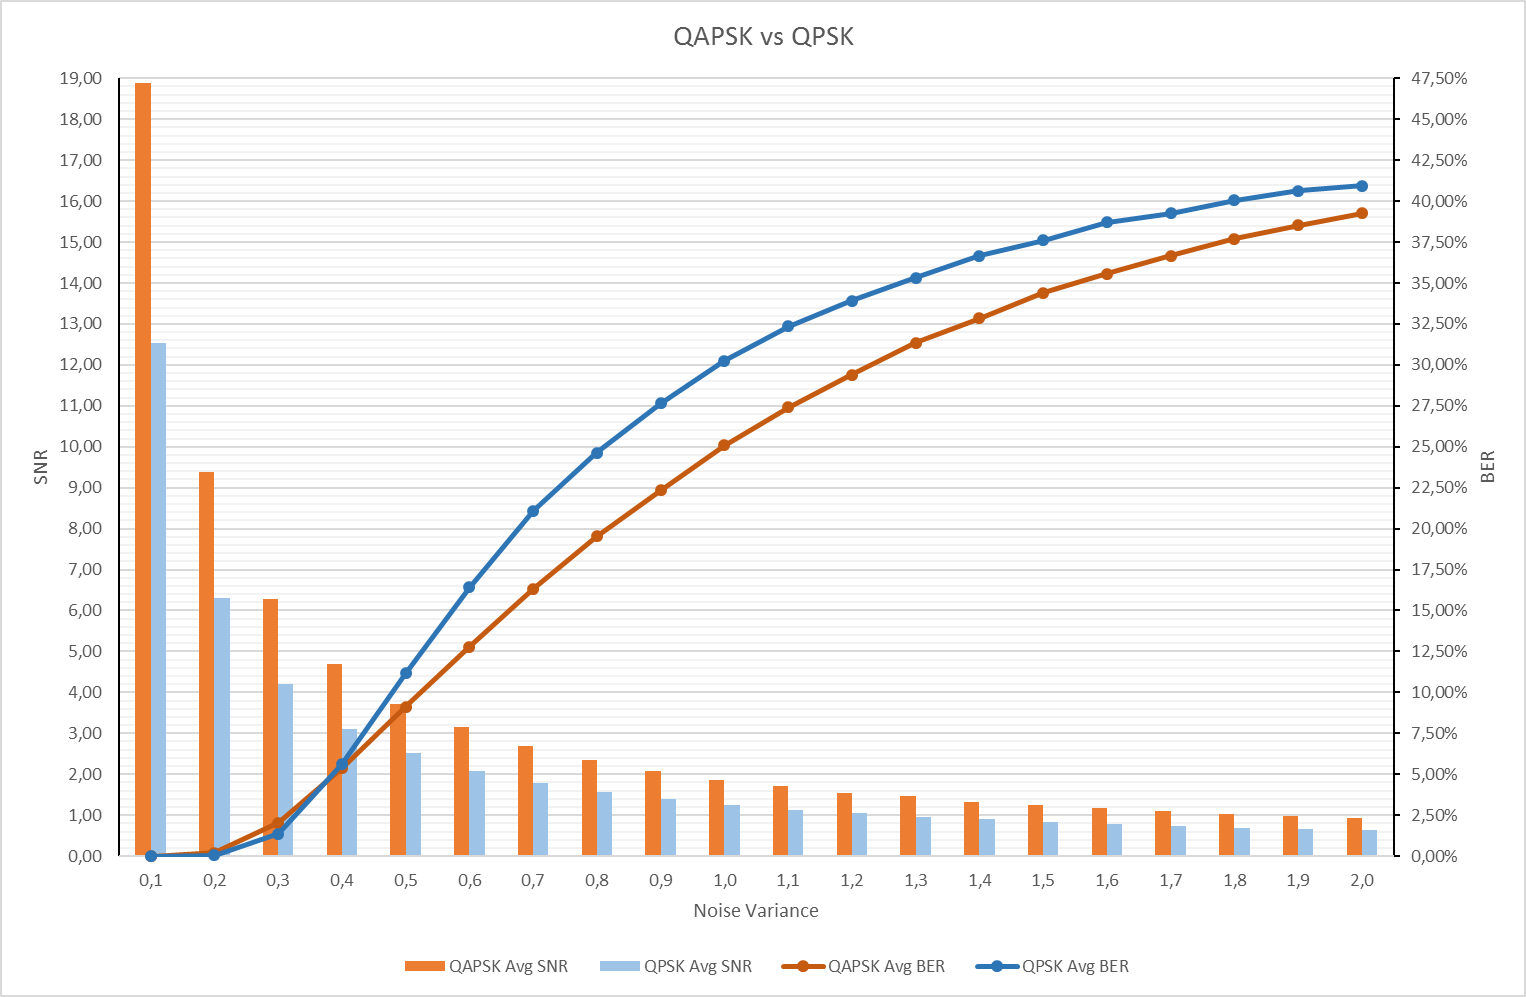
\includegraphics[width=0.8\linewidth]{img/chart/qpsk_vs_qapsk.png}
			\caption{QPSK i QAPSK, BER i SNR w funkcji amplitudy szumu}
			\label{fig:qpsk_vs_qapsk}
		\end{figure}

	\subsection{Porównanie wariantów modulacji PSK}
		\begin{figure}[H]
			\centering
			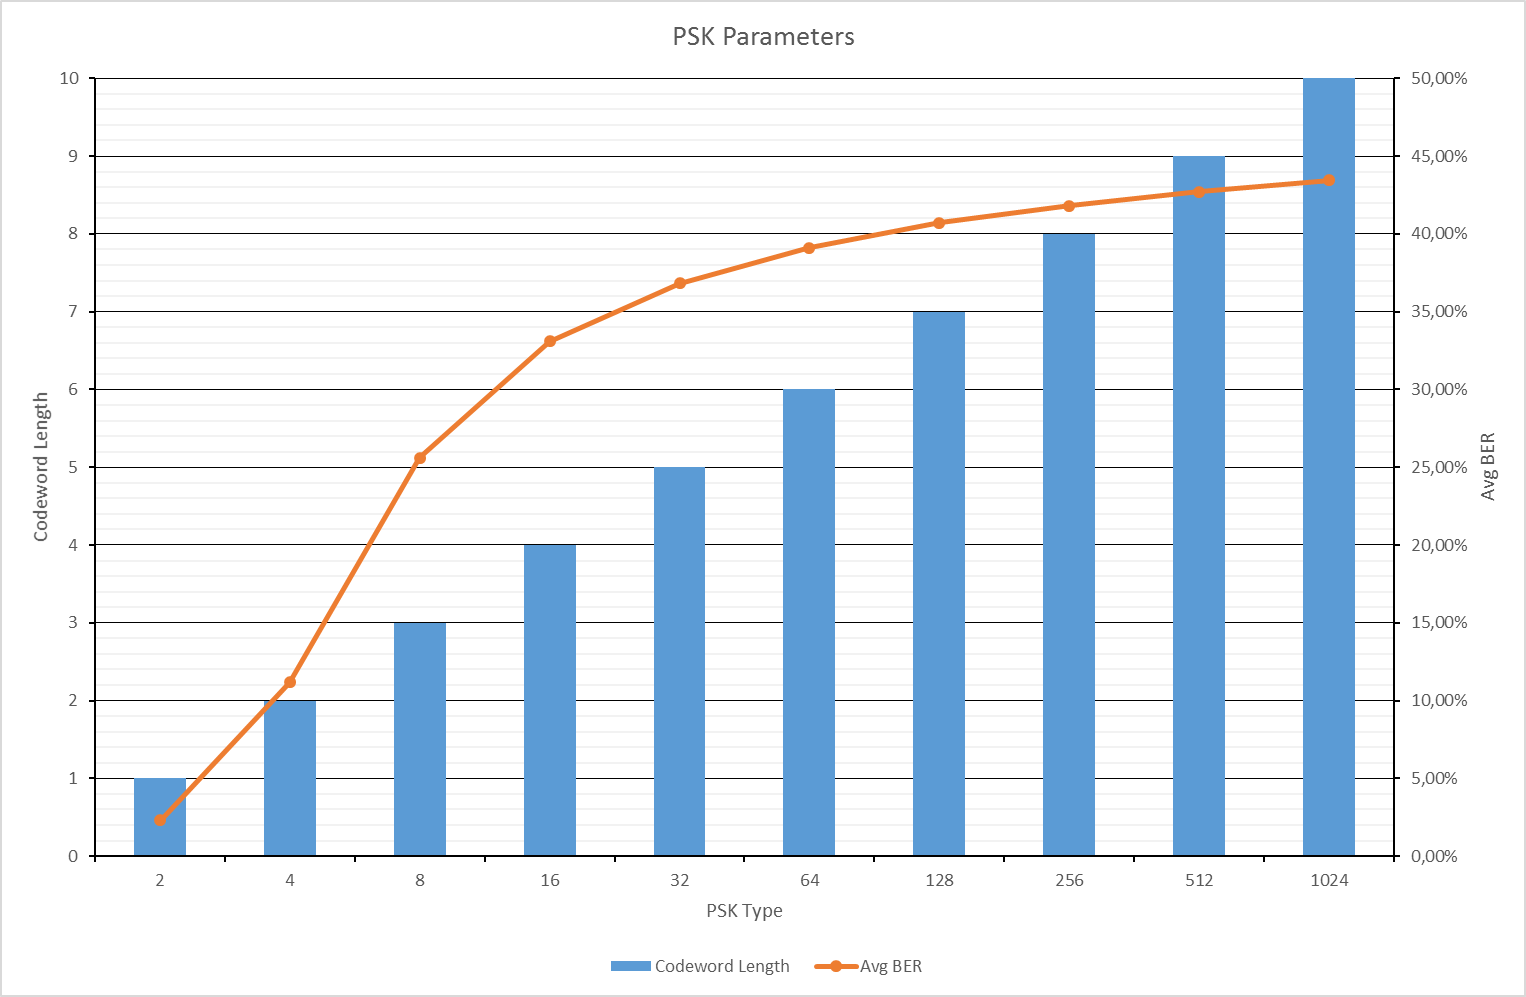
\includegraphics[width=0.8\linewidth]{img/chart/psk_comp.png}
			\caption{BER dla różnych wariantów modulacji, wariancja szumu równa 0,5}
			\label{fig:psk_comp}
		\end{figure}

\newpage
\section{Wnioski}
	Wyniki badań pokrywają się z przewidywaniami. Wzrost długości symbolu, zwiększa podatność syganału na błędy spowodowanem zakłóceniami. Wybór najlepszej metody modulacji nie jest prostym zadaniem i zalęży od wielu czynników: jakości medium transmysyjnego, zakłóceń zewnętrznych oraz potrzeb użytkowników systemu.\\

\newpage
\tableofcontents

\end{document}